\chapter{Regression}

{\sf The regression problem is the problem of minimization the sum of the squared distances between our hypothesis $h(x)$ and value $f(x)$ of datapoint $x$ ($f(x_i)$ is a label $y_i$ of a point $x_i$).}

\section{Linear and Polynomial Regression}
\vspace{-0.6cm}
\subsubsection*{Linear regression}

\begin{wrapfigure}{r}{0.3\linewidth}
	\vspace{-3cm}
  \begin{center}
    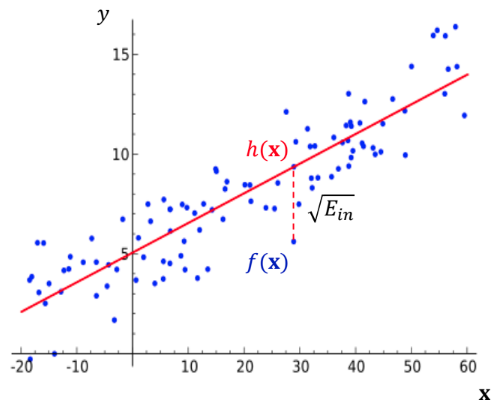
\includegraphics[width=\linewidth]{12a.png}
  \end{center}
  \vspace{-0.8cm}
  \caption*{(12.1) Linear regression}
\end{wrapfigure}
In case of linear regression we want to find optimal linear $h(x)$ ([pic. 12.1] is an example with datapoints from $\mathbb{R}$). The linear function regression corresponds to equation $h(x_i)=w^Tx_i$ (where datapoint $x_i=(a_1,\ldots,a_n)^T$ replaced by point $(1, a_1,\ldots,a_n)^T$). So we want to minimize the error $E(w)$ defined as \hyperlink{ein_and_eout}{error in sample} $E_{in}(h)$:
$$E(w)=E_{in}(h)=\frac{1}{N}\sum\limits_{i=1}^{N}(h(x_i)-f(x_i))^2=\frac{1}{N}\sum\limits_{i=1}^{N}(w^Tx_i-y_i)^2=\frac{1}{N}\|Xw-y\|_2^2$$
where
$$X=\begin{pmatrix}
	x_1^T \\
	x_2^T \\
	\ldots \\
	x_N^T \\
	\end{pmatrix} \qquad
	y=\begin{pmatrix}
	y_1 \\
	y_2 \\
	\ldots \\
	y_N \\
	\end{pmatrix}$$
And the solution is
$$\nabla E(w)=\frac{2}{N}\cdot X^T(Xw-y)=0\Rightarrow X^TXw=X^Ty\Rightarrow w=(X^TX)^{-1}X^Ty$$
Why the found solution is the minumum, not the maximum? Well, because $E(w)$ is the square of some value.

\subsubsection*{Polynomial regression}

\begin{wrapfigure}{r}{0.25\linewidth}
	\vspace{-2.5cm}
  \begin{center}
    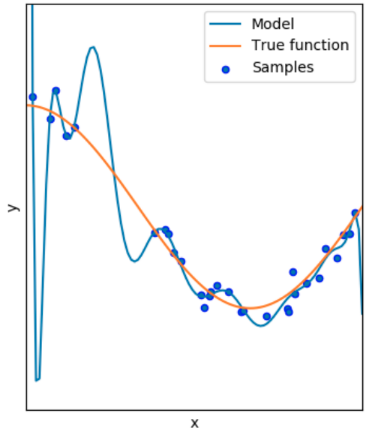
\includegraphics[width=\linewidth]{12b.png}
  \end{center}
  \vspace{-0.8cm}
  \caption*{(12.2) Overfitting}
  \vspace{-2cm}
\end{wrapfigure}
Polinomial regression is like the linear regression with polinomial features. For example:
$$x_i\in\mathbb{R},\ x_i\to(1,x_i,x_i^2)^T \qquad
x_i\in\mathbb{R}^2,\ (a_1, a_2)^T\to(1,a_1,a_2,a_1^2,a_2^2,a_1a_2)^T$$
But when we increase the dimensionality of our space, we can owerfit [pic. 12.2]. How do we fight that?

\newpage
\section{Theory of Error for Regression}
\vspace{-0.6cm}
\subsubsection*{Sine target function}

This is a simple example of linear regression of sine function:
\begin{figure}[H]
  \centering
  \begin{subfigure}[c]{0.25\linewidth}
    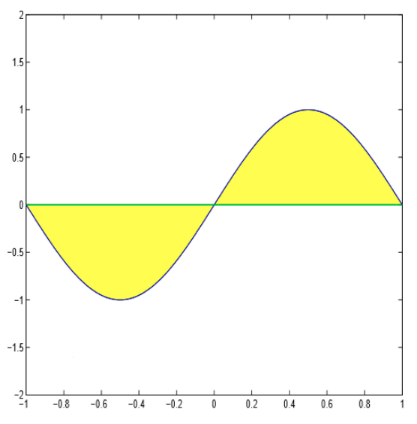
\includegraphics[width=\linewidth]{12c.png}
    \caption*{Constant hypothesis}
  \end{subfigure}
  \hspace{2cm}
  \begin{subfigure}[c]{0.25\linewidth}
    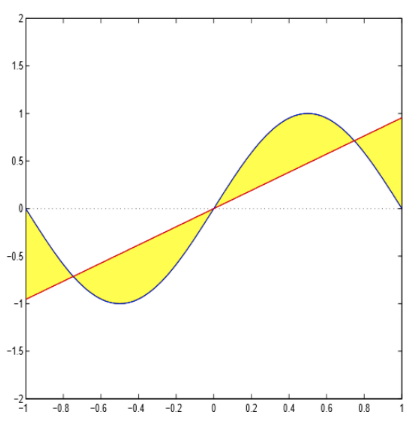
\includegraphics[width=\linewidth]{12d.png}
    \caption*{Linear hypothesis}
  \end{subfigure}
\end{figure}
The error out of sample for the first hypothesis is $0.5$ and for the second is $0.2$. Now let's say we have only two points in our dataset ([pic. 12.3] and [pic.12.4]):
\begin{figure}[H]
  \centering
  \begin{subfigure}[c]{0.26\linewidth}
    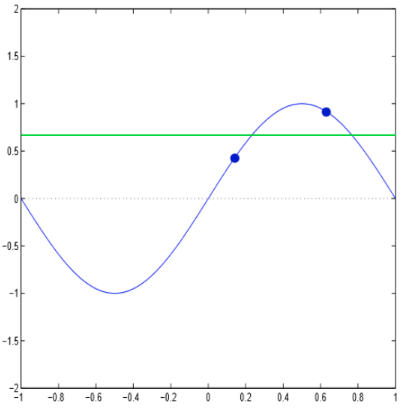
\includegraphics[width=\linewidth]{12e.png}
    \caption*{(12.3) Constant hypothesis}
  \end{subfigure}
  \hspace{1cm}
  \begin{subfigure}[c]{0.26\linewidth}
    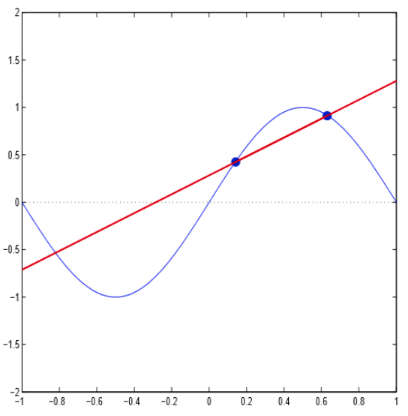
\includegraphics[width=\linewidth]{12f.png}
    \caption*{(12.4) Linear hypothesis}
  \end{subfigure}
  \hspace{1cm}
  \begin{subfigure}[c]{0.28\linewidth}
    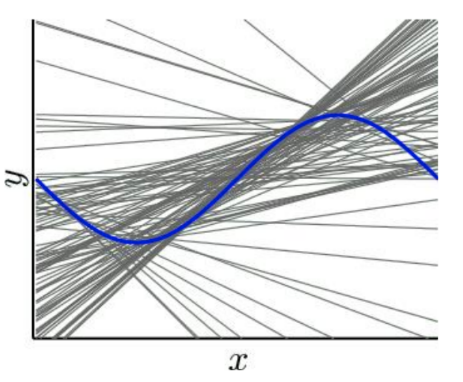
\includegraphics[width=\linewidth]{12g.png}
    \caption*{(12.5) Bad linear hypotheses}
  \end{subfigure}
\end{figure}
The error in sample for the first hypothesis is greater than zero and for the second is zero. However in the second case there is some datasets where we have big error out of sample [pic. 12.5]. To approach the theory of that we introduce mean hypothesis.

\subsubsection*{Mean hypothesis}

The error out of sample for some hypothesis $h_D$ what trained on a dataset $D$ is
$$E_{out}(h_D)=\mathbb{E}_X\left(\left(h_D(x)-f(x)\right)^2\right)$$
[Если вы забыли, что тут происходит, смотрите \hyperlink{ein_and_eout}{error out of sample}.] Now let's find the expectation of $E_{out}$ over all datasets:
$$\mathbb{E_D}\left(E_{out}(h_D)\right)=\mathbb{E}_D\left(\mathbb{E}_X\left(\left(h_D(x)-f(x)\right)^2\right)\right)=\mathbb{E}_X\left(\mathbb{E}_D\left(\left(h_D(x)-f(x)\right)^2\right)\right)$$
And the mean hypothesis is
$$\overline{h}(x)=\mathbb{E}_D\left(h_D(x)\right)$$
The interesting thing is that the mean hypothesis is very close to the best hypothesis, because $\overline{h}(x)$ is the expectation of all best hypotheses of all posible datasets. Of cource, we can't find the mean hypothesis (because it's a theoretical fucntion) but this theoretical function is close to the best hypothesis in our hypothesis set.\\
Now we have
$$\mathbb{E}_D\left(\left(h_D(x)-f(x)\right)^2\right)=\mathbb{E}_D\left(\left(h_D(x)-\overline{h}(x)+\overline{h}(x)-f(x)\right)^2\right)=$$
$$=\mathbb{E}_D\left(\left(h_D(x)-\overline{h}(x)\right)^2+\left(\overline{h}(x)-f(x)\right)^2+2\left(h_D(x)-\overline{h}(x)\right)\left(\overline{h}(x)-f(x)\right)\right)=$$
$$=\mathbb{E}_D\left(\left(h_D(x)-\overline{h}(x)\right)^2\right)+\left(\overline{h}(x)-f(x)\right)^2$$

\subsubsection*{Bias and variance}

So the $E_D\left(E_{out}(h_D)\right)$ is
$$E_D\left(E_{out}(h_D)\right)=\mathbb{E}_D\left(\mathbb{E}_X\left(\left(h_D(x)-f(x)\right)^2\right)\right)=\mathbb{E}_X\left(\mathbb{E}_D\left(\left(h_D(x)-\overline{h}(x)\right)^2\right)+\left(\overline{h}(x)-f(x)\right)^2\right)=$$
$$=\mathbb{E}_X(variance(x)+bias(x))=bias+variance$$
where
$$bias=\mathbb{E}_X\left(\left(\overline{h}(x)-f(x)\right)^2\right)$$
$$variance=\mathbb{E}_X\left(\mathbb{E}_D\left(\left(h_D(x)-\overline{h}(x)\right)^2\right)\right)$$
What does that values mean? Blue points are dataset, the hypothesis is <<points in the red circle>>:
\begin{figure}[H]
  \centering
  \begin{tabular}{cccc}
    
\includegraphics[width=0.2\linewidth]{12h.png} & \hspace{0.25cm}
    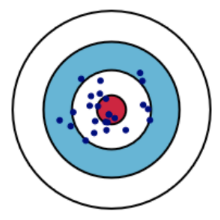
\includegraphics[width=0.2\linewidth]{12i.png} & \hspace{0.25cm}
    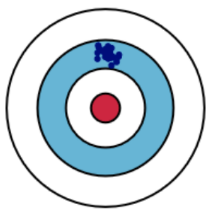
\includegraphics[width=0.2\linewidth]{12j.png} & \hspace{0.25cm}
    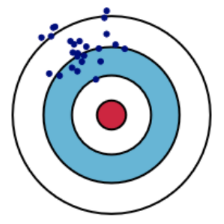
\includegraphics[width=0.2\linewidth]{12k.png} \\
    low bias & low bias & high bias & high bias \\
    low variance & high variance & low variance & high variance \\
  \end{tabular}
\end{figure}
So the error is low when bias and variance (almost) equal [pic. 12.6].\\
Here ([pic. 12.7] and [pic. 12.8]) we can see some values of bias and variance for sine target function:
\begin{figure}[H]
  \centering
  \begin{subfigure}[c]{0.36\linewidth}
    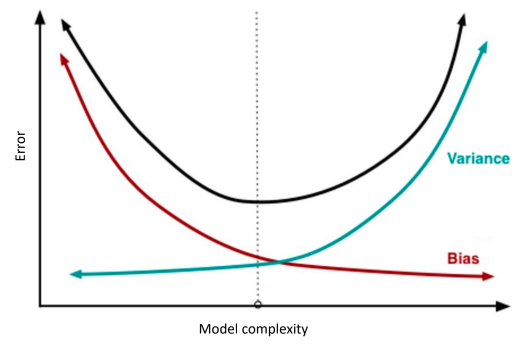
\includegraphics[width=\linewidth]{12l.png}
    \caption*{(12.6) Model complexity}
  \end{subfigure}
  \hspace{0.4cm}
  \begin{subfigure}[c]{0.28\linewidth}
    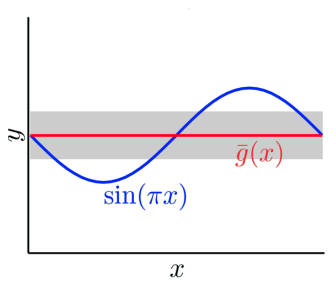
\includegraphics[width=\linewidth]{12m.png}
    \caption*{(12.7) bias=0.5 var.=0.25}
  \end{subfigure}
  \hspace{0.4cm}
  \begin{subfigure}[c]{0.28\linewidth}
    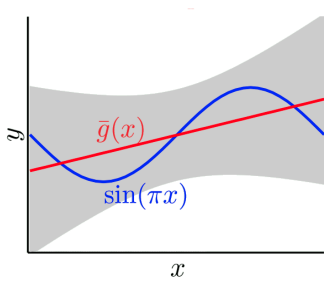
\includegraphics[width=\linewidth]{12n.png}
    \caption*{(12.8) bias=0.21 var.=1.69}
  \end{subfigure}
\end{figure}

\section{Regularization}

One of the ways to prevent overfitting is the regularization. And for regression the first way to regularize is using $L_2$ regularization.

\subsubsection*{$L_2$ regularization}

$L_2$ regularization is adding a square of the weights:
$$E(w) + \frac{\alpha}{N} w^Tw=\frac{1}{N}\|Xw-y\|_2^2+\frac{\alpha}{N} w^Tw=$$
$$=\frac{1}{N}\left((Xw-y)^T(Xw-y)+\alpha w^Tw\right)$$
$$\nabla \left(E(w)+\frac{\alpha}{N} w^Tw\right)=0\Rightarrow\left(X^TX+\alpha I\right)^{-1}X^Ty$$
Choosing $\alpha$ we have:
\begin{figure}[H]
  \centering
  \begin{subfigure}[c]{0.28\linewidth}
    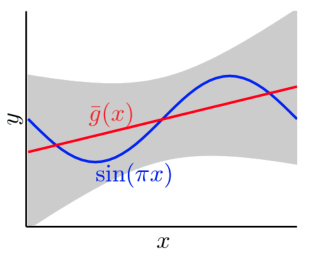
\includegraphics[width=\linewidth]{12o.png}
    \caption*{bias=0.21, var.=1.69}
  \end{subfigure}
  \hspace{2cm}
  \begin{subfigure}[c]{0.28\linewidth}
    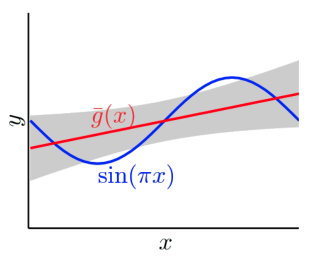
\includegraphics[width=\linewidth]{12p.png}
    \caption*{bias=0.23, var.=0.33}
  \end{subfigure}
  \vspace{-0.4cm}
\end{figure}
Big $\alpha$ ($\approx1$) is underfit because algorithms tries to made weights small rather than fitting the function.

\subsubsection*{LASSO and $L_1$ regularization}

If our feature space is greater than dataspace, we want to ignore some number of features. In that case we use LASSO (Least Absolute Shrinkage and Selection Operator). LASSO is the method what limits norm of the $w$ which makes some coefficients equal to zero. The way to do it is the $L_1$ regularization:
$$E(w)=\frac{1}{N}\|Xw-y\|_2^2+\frac{\alpha}{N}\|w\|_1$$
Now we can't optimize $E(w)$ in one step because we can't just find the derivative. So for that we use LARS (Least Angle Regression).

\subsubsection*{LARS}

Let's define $\overline{x}_i$ as a vector of the i'th features of all points from the dataset (i'th column of matrix $X$). $y$ is still the vector of labels.
\begin{enumerate}
	\item We find the feature $\overline{x}_i$ what correlates most with $y$, i.e. we find such $\overline{x}_i$ that the angle between $y$ and $\overline{x}_i$ is the smallest.
	\item Now our hypothesis is $h(x)=\pm\beta_1\overline{x}_i$ (plus if correlation between $\overline{x}_i$ and $r$ is positive, minus if it's negative). If we increase $\beta_1$, the angle between residial $r=y-h(x)$ and $\overline{x}_i$ will increase (and  the correlation between $r$ and $\overline{x}_i$ will decrease). So we change the multiplier $\beta_1$ from zero until the correlation between $r$ and $\overline{x}_i$ becomes equal to the correlation between $\overline{x}_j$ and $r$ for other feature $j$.
	\item Now our hypothesis is $h(x)=\pm\beta_1\overline{x}_1\pm\beta_2(\overline{x}_i+\overline{x}_j)$ (plus if correlation between $\overline{x}_i$ and $r$ is positive, minus if it's negative). Now we increase $\beta_2$ until the correlation between $r=y-h(x)$ and $\overline{x}_i$ becomes equal to the correlation between $\overline{x}_l$ and $r$ for some third feature $l$. Then our hypothesis will be $h(x)=\pm\beta_1\overline{x_i}\pm\beta_2(\overline{x}_i+\overline{x}_j)\pm\beta_3(\overline{x}_i+\overline{x}_j+\overline{x}_l)$... And so on.
	\item Finally we find optimal $h(x)$.
\end{enumerate}

\subsubsection*{Elastic Net}

Elastic Net is a sum of $L_1$ term and $L_2$ term:
$$E(w)=\frac{1}{N}\|Xw-y\|_2^2+\frac{\alpha(1-l)}{N}\|w\|_2^2+\frac{\alpha l}{N}\|w\|_1$$

\subsubsection*{Support vector regression machine}

SVM tries to find such line, that most points are out of margin. Now we reverse the task and we want to find such line, that most of points are in the margin [pic.]. So we have this optimization task:
$$\begin{cases}
	\frac{1}{2}\|w\|^2+C\sum(\xi_i+\xi_i^*)\to min \\
	y_i-w^Tx_i-b\le\varepsilon+\xi_i \\
	w^Tx_i+b-y_i\le\varepsilon+\xi_i^* \\
	\xi_i,\xi_i^* \ge 0 \\
\end{cases}$$
where $\varepsilon$ is the size of the margin, $\xi_i$ and $\xi_i^*$ are distances between $x_i$ and borders of the margin.

\subsubsection*{$R^2$ score}

$R^2$ score is an useful metric for regression:
$$R^2=1-\frac{u}{v}$$
where
$$u=\sum\limits_{i=1}^{N}(h(x_i)-y_i)^2\qquad v=\sum\limits_{i=1}^{N}(\overline{y}-y_i)^2\qquad \overline{y}=\frac{1}{N}\sum\limits_{i=1}^{N}y_i$$

\section{Fighting Outliers}
\vspace{-0.6cm}

\begin{wrapfigure}{r}{0.3\linewidth}
	\vspace{-2.7cm}
  \begin{center}
    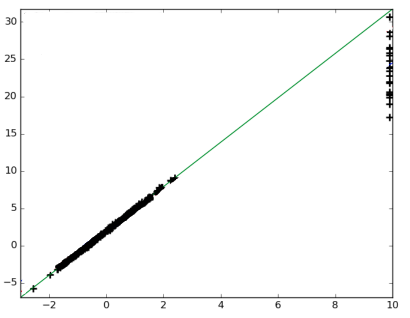
\includegraphics[width=\linewidth]{12q.png}
  \end{center}
  \vspace{-0.6cm}
  \caption*{(12.9) Theil-Sen regressor}
\end{wrapfigure}

\subsubsection*{Theil-Sen Regressor}

Let's take a subset of all points and train some number of models in that subset. The result is the marginal median of trained models [pic. 12.9].

\newpage
\subsubsection*{RANSAC (RANdom SAmple Consensus)}

\begin{wrapfigure}{r}{0.3\linewidth}
	\vspace{-2cm}
  \begin{center}
    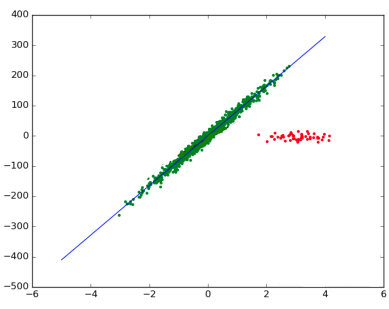
\includegraphics[width=\linewidth]{12r.png}
  \end{center}
  \vspace{-0.6cm}
  \caption*{(12.10) RANSAC}
  \vspace{-1cm}
\end{wrapfigure}
It's simular to Theil-Sen regressor: we build models on subsets of dataset. But after that we pick the best one in terms of the number of inliers (not noise points) and train a new one on all theese inliers [pic. 12.10].

\subsubsection*{Huber regressor} 

Huber regressor splits the error in two parts: close and far away points. \\
For close points we use MSE (Mean Squared Error) and for far away points we use linear error:
$$\min\limits_{w,\sigma}\sum\limits_{i=1}^{N}H_{m}\left(\frac{x_iw-y_i}{\sigma}\right)+\alpha\|w\|_2^2$$
where $\sigma$ -- scaling constant and 
$$H_m(z)=\begin{cases}
	z^2, & \text{if } |z|<\varepsilon \\
	2\varepsilon|z|-\varepsilon^2, & \text{if } |z|\ge\varepsilon
\end{cases}$$
The idea of $H_m(z)$ is the far points increase the value of the error error much more smoothly than in MSE.

\subsubsection*{Comparison of the methods}

\begin{figure}[H]
  \centering
  \begin{tabular}{cc}
    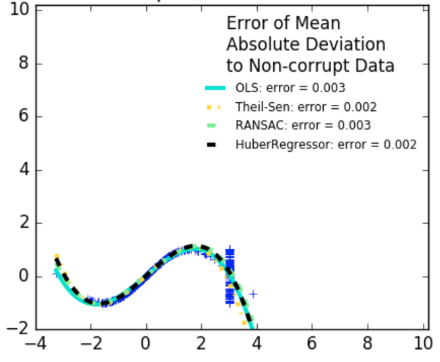
\includegraphics[width=0.35\linewidth]{12s.png} & \hspace{1cm}
    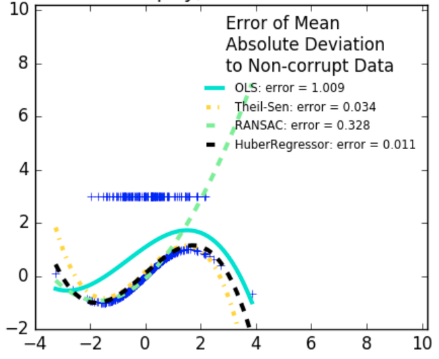
\includegraphics[width=0.35\linewidth]{12t.png} \\
    Corrupt $X$, small deviants & \hspace{1cm}
     Corrupt $y$, small deviants \\
    & \\
    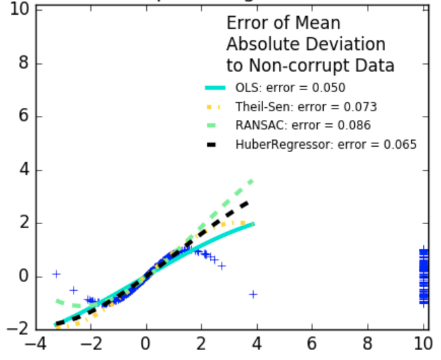
\includegraphics[width=0.35\linewidth]{12u.png} & \hspace{1cm}
    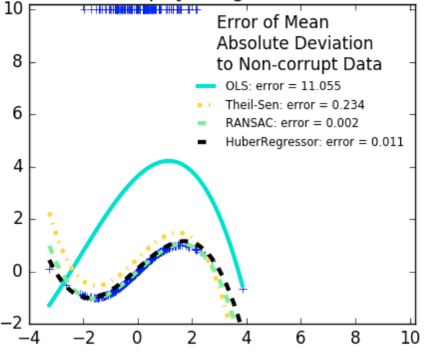
\includegraphics[width=0.35\linewidth]{12v.png} \\
    Corrupt $X$, large deviants & \hspace{1cm}
    Corrupt $y$, large deviants \\
  \end{tabular}
\end{figure}